\documentclass[14pt, fleqn, xcolor={dvipsnames, table}]{beamer}
\usepackage[T2A]{fontenc}
\usepackage[utf8]{inputenc}
\usepackage[english,russian]{babel}
\usepackage{amssymb,amsfonts,amsmath,mathtext}
\usepackage{cite,enumerate,float,indentfirst}
\usepackage{cancel}
\usepackage{graphicx}
\usepackage{animate}

\usepackage{tikz}
% \usepackage{enumitem}
\usetikzlibrary{shadows}

% \usepackage{enumitem}
% \setitemize{label=\usebeamerfont*{itemize item}%
%   \usebeamercolor[fg]{itemize item}
%   \usebeamertemplate{itemize item}}

\graphicspath{{images/}}

\usetheme{Madrid}
\usecolortheme{seahorse}
\renewcommand{\CancelColor}{\color{red}}

\setbeamercolor{footline}{fg=Blue!50}
\setbeamertemplate{footline}{
  \leavevmode%
  \hbox{%
  \begin{beamercolorbox}[wd=.333333\paperwidth,ht=2.25ex,dp=1ex,center]{}%
    И. Кураленок, Н. Поваров, Яндекс
  \end{beamercolorbox}%
  \begin{beamercolorbox}[wd=.333333\paperwidth,ht=2.25ex,dp=1ex,center]{}%
    Санкт-Петербург, 2014
  \end{beamercolorbox}%
  \begin{beamercolorbox}[wd=.333333\paperwidth,ht=2.25ex,dp=1ex,right]{}%
  Стр. \insertframenumber{} из \inserttotalframenumber \hspace*{2ex}
  \end{beamercolorbox}}%
  \vskip0pt%
}
\newcommand\indentdisplays[1]{%
     \everydisplay{\addtolength\displayindent{#1}%
     \addtolength\displaywidth{-#1}}}
\newcommand{\itemi}{\item[\checkmark]}

\newenvironment{mydescription}[1]
  {\begin{list}{}%  
   {\renewcommand\makelabel[1]{\color{blue}##1:\hfill}%
   \settowidth\labelwidth{\makelabel{#1}}%
   \setlength\leftmargin{\labelwidth}
   \addtolength\leftmargin{\labelsep}}}
  {\end{list}}

\title{Нейронные сети\\\small{совсем чуть-чуть}}
\author[]{\small{%
И.~Куралёнок,
Н.~Поваров}}
\date{}
\begin{document}

\begin{frame}
\maketitle
\small
\begin{center}
\vspace{-60pt}
\normalsize {\color{red}Я}ндекс \\
\vspace{80pt}
\footnotesize СПб, 2014
\end{center}
\end{frame}
\section{Постановка задачи и виды} % про сведение решающей функции к комбинации зависимых переменных инженерным способом

\begin{frame}{Постановка задачи обучения}{}
{\color{blue}С построением фичей}: повесим на клиента датчики \\
\textit{Наша цель повесить датчики правильно, зная какую информацию мы хотим получить.}\\
Похоже на glass box\\
~\\
{\color{blue}Без построения фичей}: льется поток неведомых данных \\
\textit{Хотим выделить сигналы, имеющие отношение к искомому} \\
Похоже на black box
\end{frame}

\begin{frame}{Пример с милиционером и бабушкой}

\end{frame}

\begin{frame}{Немного рассуждений}
\small
\textbf{А можно ли одновременно оптимизировать и выделение полезной информации и обучение?}\\
\begin{itemize}
\uncover<2->{\item Ограничимся линейными моделями как в решающей функции, так и в построении FE}
\only<2>{$$
F = \sum_i w_i \left(v_i^T x\right) 
$$}
\uncover<3->{\item Но так все сведется к линейной регрессии! Давайте добавим какое-нибудь нелинейное преобразование}
\only<3>{$$
F = \sum_i w_i g\left(v_i^T x\right)
$$}
\uncover<4->{\item Если преобразование монотонное, то можно его для красоты применить и к результату}
\only<4>{$$
F = g\left(\sum_i w_i g\left(v_i^T x\right)\right)
$$}
\uncover<5->{\item Дополним рекурсией и будем подбирать не одну функцию а несколько}
\only<5->{$$
F_i = g\left(\mathbf{w}_{di}^T g(W_{d-1}g(\ldots g(W_{0}x))\right)
$$}
\end{itemize}
\uncover<6->{$\Rightarrow$Понятно, что так писать не удобно.}
\end{frame}

\begin{frame}{Персептрон Розенблатта}
\small
$$
F_i = g\left(\mathbf{w}_{di}^T g(W_{d-1}g(\ldots g(W_{0}x))\right)
$$
Как можно видеть, система состоит из некоторого количества блоков $g(W_tu)$. Если блок 1, $g = sign(x)$ и мы подбираем одну функцию, то
\begin{center}
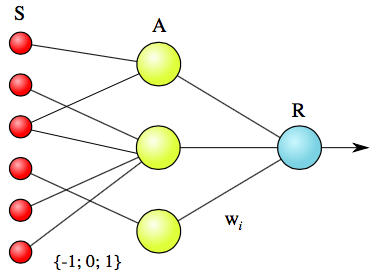
\includegraphics[width=0.4\textwidth]{Simple_perceptron}
\end{center}
это элементарный персептрон Розенблатта. Если блоков много, то сложный :).
\end{frame}

\begin{frame}{Немного истории}
\begin{enumerate}
  \item ``кибернетическая модель мозга'' 1957
  \item ЭВМ Mark I 1960
  \item Minsky, Papert ``Perceptrons: an introduction to computational geometry'' 1969
  \item Mark III 1985
  \item Krizhevsky, A., Sutskever, I. and Hinton, G. E. ``ImageNet Classification with Deep Convolutional Neural Networks''
\end{enumerate}

\end{frame}

\begin{frame}{Типы нейро компьютеров}
\begin{center}
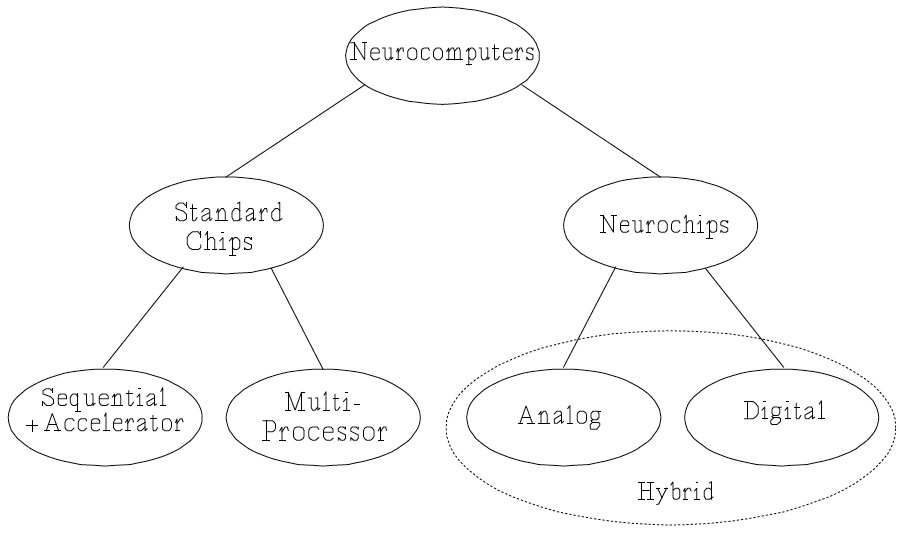
\includegraphics[width=0.8\textwidth]{neurocomp-types}
\end{center}
\end{frame}

\section{Биология и основные понятия} % подробно про функции разных кусков
\begin{frame}{}
\begin{center}
\Huge
Но на самом деле все было не так!
\end{center}
\end{frame}

\begin{frame}{Виды нейронных сетей}
C FE и без FE
Способ взаимодействия нейронов: с обратной связью, без, по соседям

\end{frame}

\section{Персептронные сети и обратное распространение ошибки} % понятие персептрона, BP, расширения персептронных сетей W-нейроны и прочая херня
\begin{frame}{Поняте персептрона}
\end{frame}


\section{Ассоциотивная память} % Сети Хопфилда, Bolzman machine

\begin{frame}{Что мы сегодня узнали}
\begin{itemize}
  \item Можно решать задачи обучения в комплексе
  \item Есть прямые аналогии в биологии (культ карго) и этим пробовали пользоваться
  \item Это сложно (получается при большой удаче) и для этого есть специальный язык
  \item Есть разные принципы построения взаимодействия внутри сети
  \item Природа все равно без датчиков не живет
\end{itemize}
\end{frame}
\end{document}
